\chapter{Neural Network Configuration}
\label{chapter:hyper}
\section{Hyperparameter Optimization I}

Fig.\,\ref{fig:hyperband_resnet_params} provides a summary of the search space for the initial hyperparameter tuning process and its results. These parameters are critical as they influence the model's learning process, generalization ability, and susceptibility to issues such as overfitting or bias. The chosen values in the search space represent a balance between exploring a wide range of options and focusing on promising areas based on prior knowledge or domain-specific considerations.

\begin{figure}[ht]
    \centering
    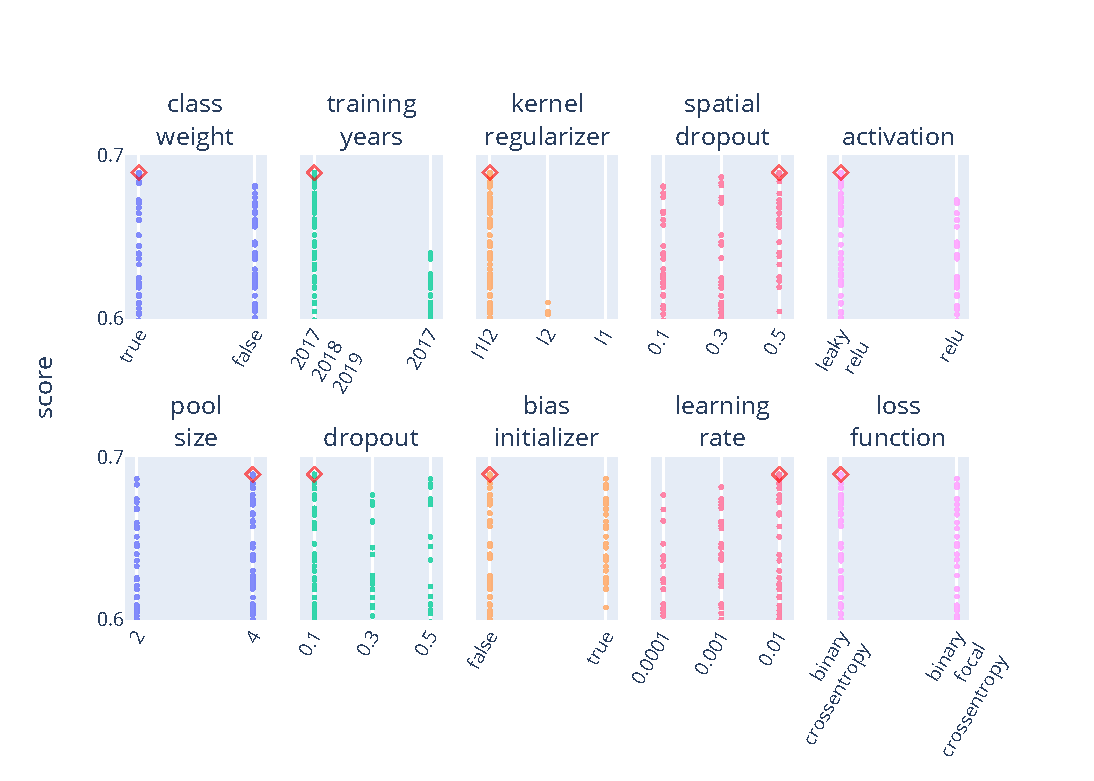
\includegraphics[width=0.9\linewidth, trim={10pt 10pt 15pt 40pt}, clip]{figures/figures_tuner/hyperband_resnet_params.pdf}
    \caption{The top f2-scores out of nearly 700 Hyperband (\cite{hyperband}) trials. The best score is marked by a diamond shape.}
    \label{fig:hyperband_resnet_params}
\end{figure}

The most successful trial values are marked by a diamond shape in Fig.\,\ref{fig:hyperband_resnet_params}. While some of the initial trial's hyperparameters do not show significant overall improvement, some parameters such as class weight, training years, and kernel regularizer do stand out. 

\section{Hyperparameter Optimization II}

A second hyperparameter tuning process was conducted using the best values from the most successful initial trial. This set of trials focused on optimizing the number of layers, the filter size of the convolutional layers, and the number of units in the fully connected (dense) layers.

\begin{figure}[ht]
    \centering
    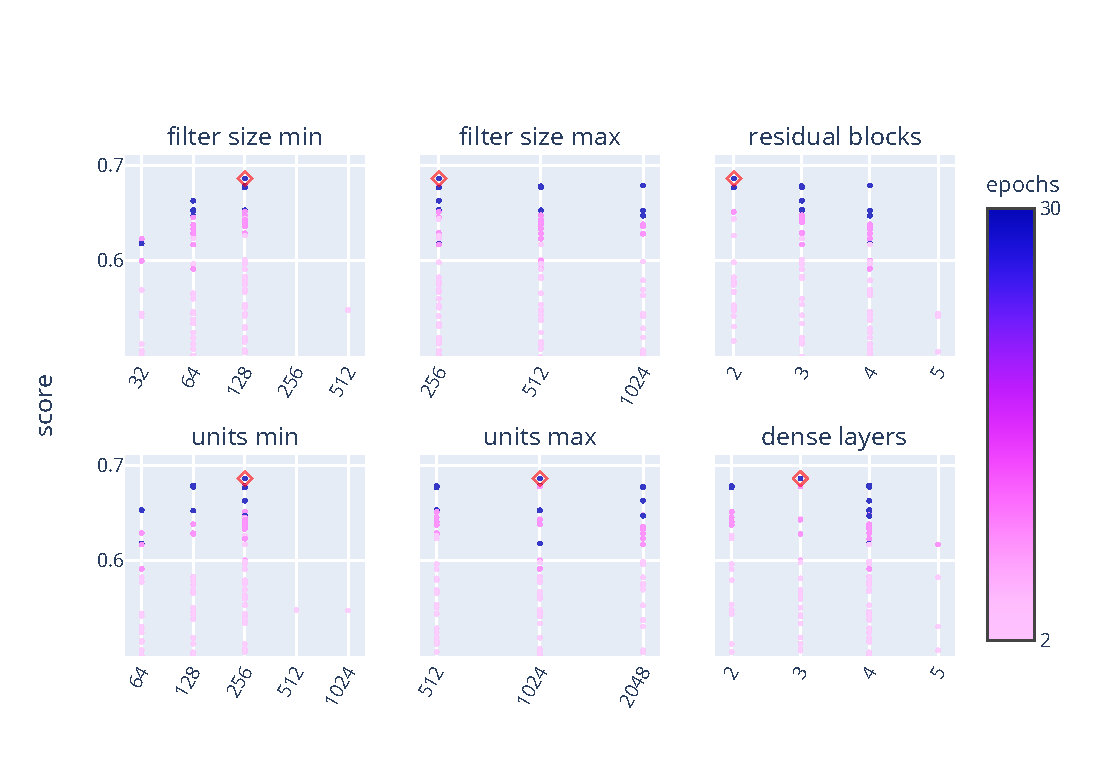
\includegraphics[width=0.9\linewidth, trim={10pt 10pt 15pt 40pt}, clip]{figures/figures_tuner/hyperband_resnet_followup_params.pdf}
    \caption{The top f2-scores for the initial hyperparameter tuning process are highlighted, with the best score marked by a diamond shape.}
    \label{fig:hyperband_resnet_followup_params}
\end{figure}

Fig.\,\ref{fig:hyperband_resnet_followup_params} illustrates the results of the second set of trials. In these trials, the minimum and maximum values for the units in each layer were varied according to predefined options, which are shown on the x-axis. Layers were generated based on these minimum and maximum values, as well as on intermediate multiples of 2. For instance, with a maximum of 1024 units and a minimum of 256, an additional layer with 512 units was created, resulting in a dense block with three layers. Notably, this configuration, represented by the diamond shapes in Fig.\,\ref{fig:hyperband_resnet_followup_params}, was identified as the optimal dense layer combination. The number of residual blocks followed a similar logic. 

\section{Model Architecture}

\begin{figure}[ht]
    \centering
    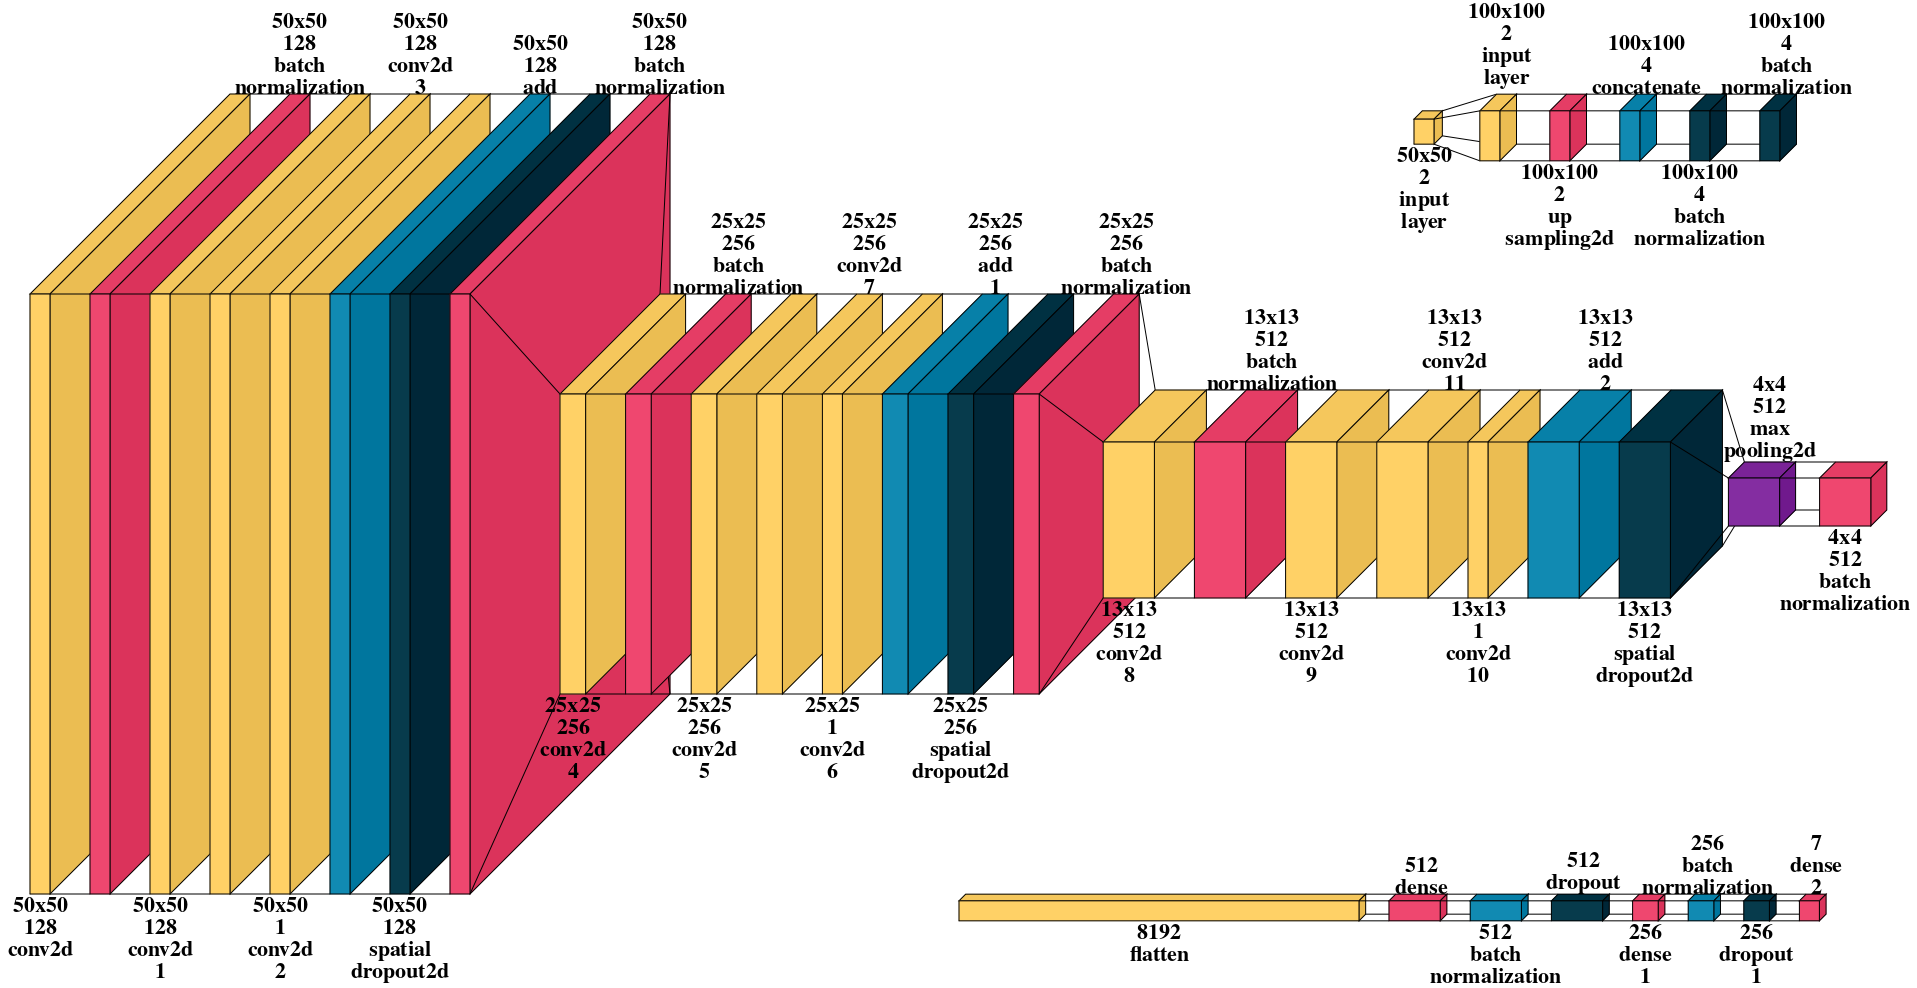
\includegraphics[width=0.9\linewidth]{figures/figures_tuner/model_layered_view.png}
    \caption{The model's layered architecture is depicted. The top-right shows the input layers, the middle section displays the convolutional layers, and the bottom-right illustrates the fully-connected layers. The layered views were generated using VisualKeras, \cite{visualkeras}.}
    \label{fig:model_layered_view}
\end{figure}

Fig.\,\ref{fig:model_layered_view} illustrates the detailed architecture of the deep learning model built using the results of the hyperparameter tuning processes. The figure highlights the flow of data through its various layers. The model starts with input layers, which include upsampling layers to handle inputs with different dimensions. This ensures that all input sources are properly aligned for processing within the model. The network then progresses through multiple convolutional layers, with filter sizes generally increasing as the layers deepen. Batch normalization and dropout layers are strategically placed to regularize the model and reduce overfitting.

The architecture incorporates residual connections for maintaining gradient flow during backpropagation. These connections enable the network to be deep without suffering from issues like vanishing gradients, as highlighted in \cite{resnet}. As the network advances, spatial dimensions are reduced through pooling and striding operations, leading to a flattening layer that prepares the data for the dense layers. These dense layers further reduce the dimensionality, eventually outputting a 7-dimensional vector corresponding to the classification into 7 different tree genera, aligning with the model's goal of predicting tree types.



